\usetikzlibrary{decorations.pathreplacing}

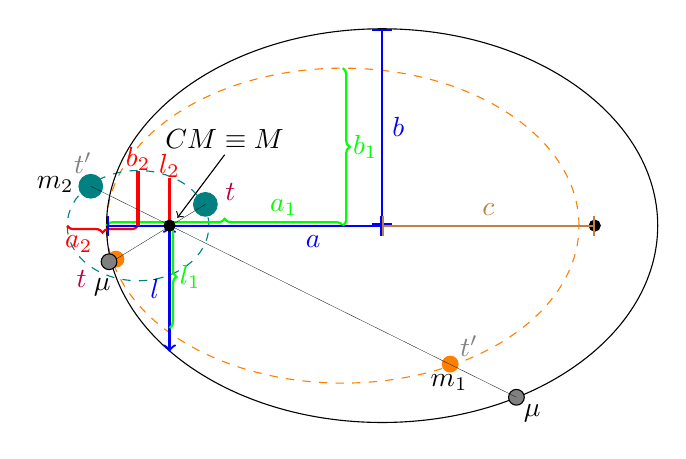
\begin{tikzpicture}

\draw [orange, dashed] (-2,0.5) node (v5) {} ellipse (3 and 2);
\draw [teal, dashed] (-4.6,0.5) node (v6) {} ellipse (0.9 and 0.7);
\draw [fill] (-4.2,0.5) node (v10) {} circle (0.05);
\node at (-3.5,1.6) {$CM\equiv M$};
\draw [fill, teal]  (-5.2,1) node (v3) {} circle (0.15);
\draw  [fill, orange](-0.6348,-1.2583) node (v4) {} circle (0.1);
\draw [fill, teal] (-2.9,0.5) node (v1) {} circle (0);
\draw [fill, orange] (-5,0.5) node (v2) {} circle (0);
\draw [->] (-3.5,1.4) -- (-4.1,0.6);
\node [purple] at (-5.3175,-0.1813) {$t$};
\node [gray] at (-5.3,1.3) {$t'$};
\node [purple] at (-3.4278,0.9226) {$t$};
\node [gray] at (-0.3965,-1.0297) {$t'$};
\node at (-5.6512,1.0265) {$m_2$};
\node at (-5.0539,-0.2816) {$\mu$};
\draw [thin] (-1.5,0.5) node (v7) {} ellipse (3.5 and 2.5);
\node at (0.4058,-1.8797) {$\mu$};
\draw  [fill=gray](0.2058,-1.6797) circle (0.1);
\draw[decorate, decoration=brace, draw=red, thick] (-4.6,0.5) -- (-5.5,0.5) node [midway, below left, red]{$a_2$};
\draw[decorate, decoration=brace, draw=green, thick] (v2.center) -- (v5.center) node [near end, above, green]{$a_1$};
\draw [thick, blue,|-|](v7.center) -- (-5,0.5) node [near start, below, blue]{$a$};
\node (v9) at (-4.6,1.2) {};
\node (v8) at (-2,2.5) {};
\draw[red, very thick] (v6.center) -- (v9.center) node [midway, above=6, red]{$b_2$};
\draw[decorate, decoration=brace, draw=green, thick] (v8.center) -- (v5.center) node [midway, right, green]{$b_1$};
\draw [thick, blue,|-|](v7.center) -- (-1.5,3)node[midway, right, blue]{$b$};
\draw [thick, blue,<->](-4.2,0.5) -- (-4.2,-1.1)node[midway, left, blue]{$l$};
\draw [decorate, decoration=brace, draw=green, thick] (v10.center) -- (-4.2,-0.8)node[midway, right, green]{$l_1$};
\draw [red, very thick](-4.2,1.1) -- (v10.center)node [midway,above=5, red]{$l_2$};
\draw  [fill](1.2,0.5) node (v11) {} circle (0.07);
\draw [thick, brown, |-|] (-1.5,0.5) -- (v11.center)node [midway, above]{$c$};
\draw  [fill](v10) circle (0.07);
\draw [fill, teal] (-3.7445,0.7701) node (v12) {} circle (0.15);
\draw [fill, orange] (-4.8801,0.0743) node (v13) {} circle (0.1);
\draw [ultra thin](v12.center) -- (v13.center);
\draw[ultra thin] (v3.center) -- (0.2058,-1.6797);
\node at (-0.6496,-1.492) {$m_1$};
\draw  [fill=gray](-4.9678,0.0415) circle (0.1);
\end{tikzpicture}